% \documentclass[11pt,twoside,a4paper,titlepage]{article}
\documentclass[10pt,twoside,a4paper,titlepage]{article}
%%%%%%% Standard settings %%%%%%%
\usepackage{amsmath}
\usepackage{amssymb}
\usepackage[nottoc, numbib, notlot, notlof]{tocbibind}
\usepackage{fancyhdr}
\usepackage[english]{babel}
\usepackage[utf8]{inputenc}
\usepackage{microtype}
\usepackage[svgnames]{xcolor}
\usepackage{siunitx}
\usepackage{tabularx}
\setlength{\headheight}{15pt}
\usepackage{footnote}
\setcounter{tocdepth}{2} % Number of layers in table of content
\setcounter{secnumdepth}{5} % number of layers in sections
\usepackage[toc,page]{appendix} % appendices
% \usepackage{gensymb}% Adds a \degree symbol in math mode
\usepackage{chngcntr}
\counterwithin{figure}{section}
\counterwithin{table}{section}
\counterwithin{equation}{section}
% % Two paged margin:
% \usepackage[margin=2.5cm, inner =3cm,outer =2cm]{geometry}
% % One paged magin:
\usepackage[margin=2.5cm]{geometry}
\usepackage{paralist}
\let\itemize\compactitem
\let\enditemize\endcompactitem
\let\enumerate\compactenum
\let\endenumerate\endcompactenum
\let\description\compactdesc
\let\enddescription\endcompactdesc
\pltopsep=1pt
\plitemsep=1pt
\plparsep=1pt
%%%%%%% FIGURES %%%%%%%
\usepackage{tikz}
% \usepackage{tikz-timing}
% \usepackage[americanvoltages, americancurrents, americanresistors, americaninductors, smartlabels]{circuitikz}
\usetikzlibrary{positioning} % in the preamble
\usetikzlibrary{decorations.pathreplacing}
\usetikzlibrary{arrows,shapes,automata}
\usepackage{graphics}
\usetikzlibrary{shapes,chains, scopes}
\usepackage{pgfplots}
\usepackage{tabu}
\pgfplotsset{compat=1.8} % Should be supported on all machines.
\usepackage{graphicx} % used for MATLAB figures in the format .eps
\usepackage{epstopdf} % Used for automatic convertion of .eps to pdf; Without this we cannot compile with pdfLaTeX.
\usepackage{epsfig}
\usepackage{subcaption}

\usepackage{pdflscape} %% to make landscape. The same as lscape but rotated for viewing the side normally in a pd

%%%%%%% captions settings %%%%%%%
\usepackage{caption}
\captionsetup{font=footnotesize}

%Figure text under code snippits
%%%%%%% Misc %%%%%%%
\usepackage{icomma}
\usepackage{pdfpages}
\usepackage[pdftex,
hyperfigures=true,
pdfauthor={Authors},
pdftitle={},
pdfsubject={},
pdfkeywords={},
hidelinks,
plainpages=false,
pdfpagelabels,
unicode]{hyperref}
\usepackage{textcomp} 
\newenvironment{changemargin}[2]{%
\begin{list}{}{%
\setlength{\topsep}{0pt}%
\setlength{\leftmargin}{#1}%setlength{\rightmargin}{#2}%
\setlength{\listparindent}{\parindent}%
\setlength{\itemindent}{\parindent}%
\setlength{\parsep}{\parskip}%
}%
\item[]}{\end{list}}

\usepackage{xcolor,colortbl}
\newcommand{\mycheckmark}{\includegraphics[width=0.7cm]{./graphics/checkmark}}
\definecolor{Green}{rgb}{0.04,0.45,0.11}

%individual todo notes
\usepackage[disable]{todonotes}

\usepackage{color}
\usepackage{nameref}
\makeatletter
\newcommand*{\currentname}{\@currentlabelname}
\makeatother

\newcommand{\nikolaj }[1]{\todo[inline, color=red!50   ]{\currentname: #1}}
\newcommand{\thomas  }[1]{\todo[inline, color=red!20   ]{\currentname: #1}}
\newcommand{\david   }[1]{\todo[inline, color=orange!20]{\currentname: #1}}
\newcommand{\xabier  }[1]{\todo[inline, color=green!20 ]{\currentname: #1}}
\newcommand{\kirstine}[1]{\todo[inline, color=green!50 ]{\currentname: #1}}
\newcommand{\casper  }[1]{\todo[inline, color=blue!20  ]{\currentname: #1}}
\newcommand{\simon   }[1]{\todo[inline, color=blue!50  ]{\currentname: #1}}

%gantt charts... I use them in a tabular...
\newcommand{\ganttScaling}{0.2}
\newcommand{\ganttLine}[3]{\begin{tikzpicture}[scale=\ganttScaling] \draw[line width=2mm,color=#1] (0,0) ( #2,0)  --    ++(  #3,0);  \end{tikzpicture}}
% Color - Start - Duration

%Should be used in every controller diagram - anbae12.

\tikzstyle{block} = [draw, fill=blue!20, rectangle, minimum height=2.5em, minimum width=4em]
\tikzstyle{blockgreen} = [draw, fill=green!40, rectangle, minimum height=2.5em, minimum width=4em]
\tikzstyle{blockorange} = [draw, fill=orange!60, rectangle, minimum height=2.5em, minimum width=4em]
\tikzstyle{blocknon} = [draw, rectangle, minimum height=2.5em, minimum width=4em]
\tikzstyle{freq} = [draw, fill=green!20, ellipse, minimum height=2.5em, minimum width=3.5em]
\tikzstyle{sum} = [draw, fill=blue!20, circle, node distance=1cm]
\tikzstyle{input} = [coordinate]
\tikzstyle{output} = [coordinate]
\tikzstyle{pinstyle} = [pin edge={to-,thin,black}]

\tikzstyle{zero} = [scale = 0.2, draw, circle, minimum width=1cm, thick]
\tikzstyle{pole} = [scale = 0.2, draw, cross out, minimum width = 1cm, minimum height=1cm, thick]

\begin{document}
% Disable indentation
\setlength{\parindent}{0pt}
\setlength{\parskip}{0.7\baselineskip}%
\pagenumbering{gobble}
\thispagestyle{empty}
%\begin{titlepage}


\title{Phase 1}
\author{Nikolaj, Thomas, David, Xabier, Kirstine \& Simon }
\date{December 2014}

\begin{figure}[b]
\centering
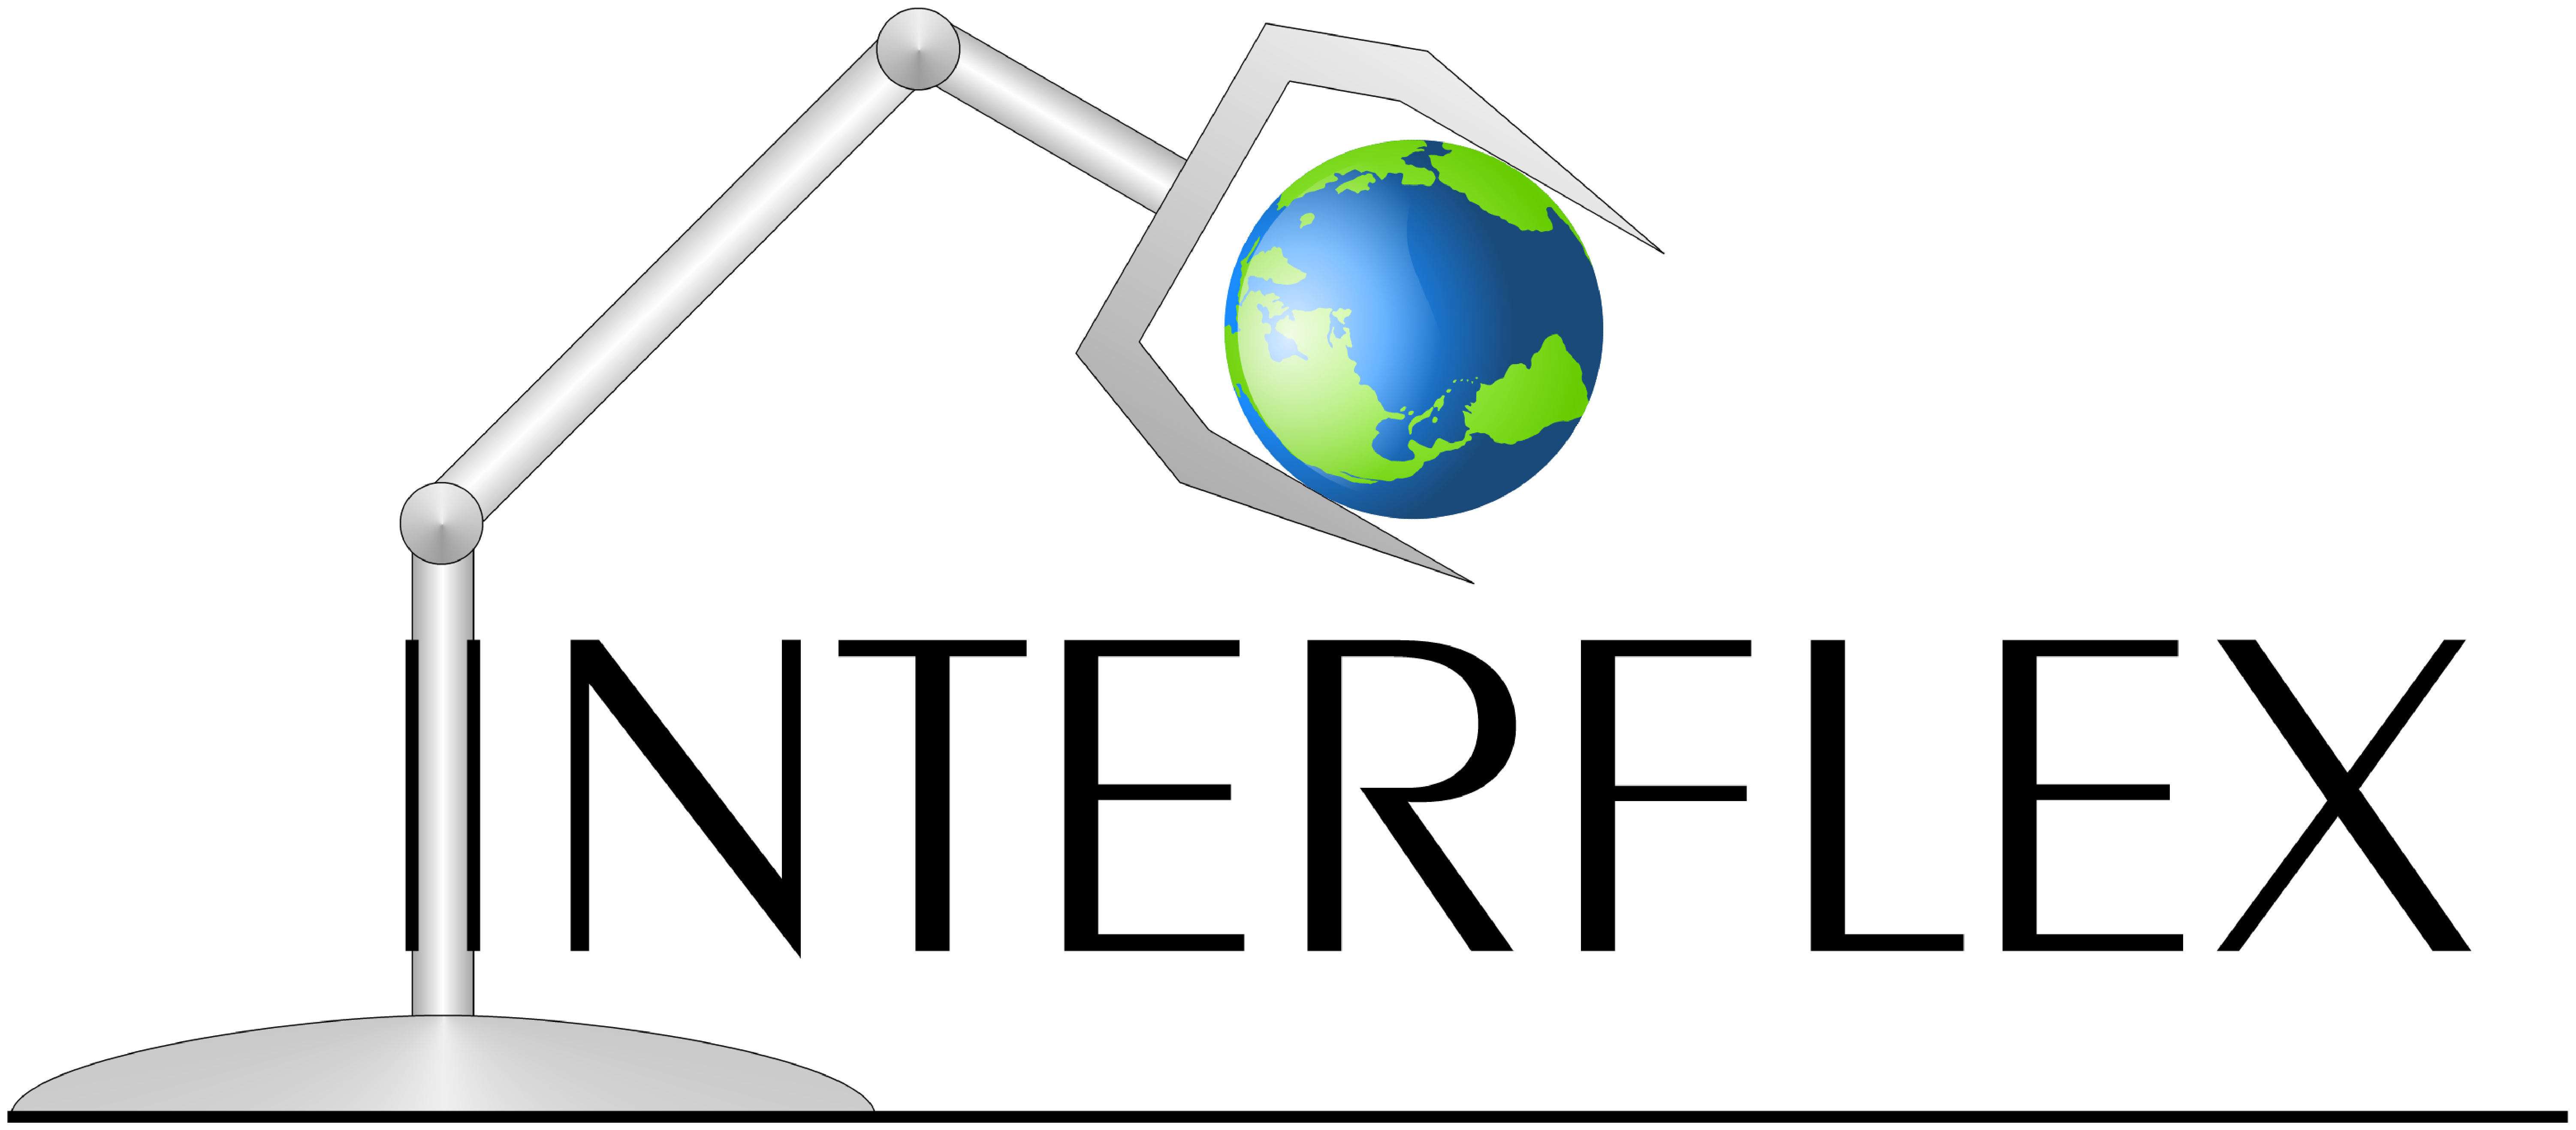
\includegraphics[width=0.4\textwidth]{graphics/logo}
\end{figure}

\vfill
\end{titlepage}
\maketitle

\clearpage
\fancyfoot{}
\fancyfoot[CO,CE]{\thepage}
\pagenumbering{Roman}

% \section{Important information to everyone}
% I have noticed an inconsistent use of todo notes.
% To adjust for this I have made a shortcut for everyone so we can see who wrote it and it uses the same syntax.
% Just write
% \begin{verbatim}
% \name{note}          
% \end{verbatim} and the title of the section will be put in and a color will be chosen for each person.
% \nikolaj {nikolaj }
% \thomas  {thomas  }
% \david   {david   }
% \xabier  {xabier  }
% \kirstine{kirstine}
% \casper  {casper  }
% \simon   {simon   }

%%%%% Formalia should go here %%%%%%%

% \setcounter{page}{1}
\section*{Abstract}
This is where we would write our actual abstract. 
This should be clear that this is a placeholder and not the real abstract.
When we get further we should obviously write a serious one. 
\newpage
\tableofcontents
\clearpage
\listoffigures
\listoftables
\listoftodos

\pagestyle{fancy}
\fancyfoot{}of December at 12:15-13:00
\pagenumbering{arabic}
\setcounter{page}{1}
\fancyfoot[LO,RE]{\thepage}

%%%%% Content should go here %%%%%%%
\section{Collaboration}

%Introduction to Collaboration

Throughout the project the group has done several activities to improve and strengthen the collaboration. 
Good collaboration is crucial for several different reasons. 
First, it is important that we can identify each others strengths and weaknesses, so that we know which areas to have in mind when cooperating. 
Knowing each others personalities helps us collaborate. 
If everyone is comfortable expressing their opinion a better product will come out in the end. The things that have been done to improve collaboration are listed and described in this section. 


\subsection{Reflections on Use of the Group Contract}

A copy of the group contract is to be found in appendix \ref{app:groupContract}

In this group, we have different experienceses with groupwork, some more positive than others, but we all agreed that we wanted to take this project seriously. For this reason we found the group contract redundant. 
The main points we decided to put into the contract was that everyone had to show up on time for group meetings, or at least let the group know they were late. We also decided on an agenda for group meetings. The consequence of not following the rules are that a warning will be given, and if no improvement a second warning could kick you out of the group. 

This is a sensible group contract if everyone is serious and commited to the project, but then it is redundant anyway. It was decided in the group that this was good enough for us. 

Throughout this project we have had problems communicating and getting everyone to attend. The meetings have been weakly defined and chaotic. 
Looking back, we should have been much more specific in making the group contract. It should have had more concrete consequences to be late to a meeting, or to not meet deadlines. There should also have been a guideline to figure out who should write the summeries of the group meethings, etc. 

One thing that could have helped was to have a system where if you are late, you pay a fee, or bring cake or something. This would give the small violations of the rules a small consequence. 
For the group meetings, it would have been a good idea to have a group leader and a secretary, so there was always someone who made sure to follow the agenda, and someone who wrote everything down. This could be either changing from each meeting or different people every time. A good idea would be to use the Belbin profiles to choose who should have which roles. 

Other details, like which programs the report should be written in, and which programs should be used to store it, could also have been added, to avoid any confusion. 

In hindsight, stating a more concise group contract, and following it, could have benefitted the group.

\subsection{Competence triangle}

\tikzstyle{theo} = [font=\footnotesize, rotate=60,  draw, rectangle, fill=blue!10, text=black, text width = 3.7em, minimum height =4.1em, text centered, node distance=1.7cm]
\tikzstyle{exp} =  [font=\footnotesize, rotate=-60, draw, rectangle, fill=blue!10, text=black, text width = 3.7em, minimum height =4.1em, text centered, node distance=1.7cm]
\tikzstyle{pers} = [font=\footnotesize,             draw, rectangle, fill=blue!10, text=black, text width = 3.7em, minimum height =4.1em, text centered, node distance=1.7cm]

\begin{figure}[!ht]
\centering
\begin{tikzpicture}[scale=0.7, every node/.style={scale=0.7}]
\node[draw, very thick, regular polygon,regular polygon sides = 3, minimum width= 7cm] (strengths) at (0,0) {};

\node[rotate=60, yshift=-0.5cm, xshift=-0.3cm] (theoretical) at (strengths.135) {Theoretical knowledge};
\node[rotate=-60, yshift=-0.5cm, xshift=0.3cm] (experience) at (strengths.40) {Work skills and Experiences};
\node[yshift=0.5cm] (personal) at (strengths.270) {Personal strengths};

\node[theo, above of=theoretical, yshift = -0.2cm, xshift=-3cm] (ta) {Software development (4)} ;
\node[theo, right of=ta] (tb)                                        {Electrical circuits} ;
\node[theo, right of=tb] (tc)                                        {Databases} ;
\node[theo, right of=tc] (td)                                        {Maths (3)} ;
\node[theo, above of=ta, xshift=-2.5em, yshift=-0.2cm] (te)          {Control theory} ;
\node[theo, right of=te] (tf)                                        {Energy} ;
\node[theo, right of=tf] (tg)                                        {C++ programming (2)} ;
\node[theo, right of=tg] (th)                                        {C programming (3)} ;
\node[theo, right of=th] (ti)                                        {Java programming (1)} ;
\node[theo, above of=te, xshift=-2.5em, yshift=-0.2cm] (tj)          {Physics} ;
\node[theo, right of=tj] (tk)                                        {Mechanics} ;
\node[theo, right of=tk] (tl)                                        {RE tech} ;
\node[theo, right of=tl] (tm)                                        {Lasers} ;
% \node[theo, right of=tm] (tn)                                        {Waves} ;
\node[theo, right of=tm] (to)                                        {Process management} ;
\node[theo, right of=to] (tp)                                        {Computer simulation} ;

\node[exp, above of=experience, yshift = -0.2cm,xshift=-7.4em] (ea) {Teaching non experts} ;
\node[exp, right of=ea] (eb)                                      {Auto\-mation} ;
\node[exp, right of=eb] (ec)                                      {Debating} ;
\node[exp, right of=ec] (ed)                                      {Wind turbines} ;
\node[exp, above of=ea, xshift=-2.5em, yshift=-0.1cm] (ee)        {Explo\-rative} ;
\node[exp, right of=ee] (ef)                                      {Program\-ming} ;
\node[exp, right of=ef] (eg)                                      {Planning} ;
\node[exp, right of=eg] (eh)                                      {Control} ;
\node[exp, right of=eh] (ei)                                      {Carpentry} ;
\node[exp, above of=ee, yshift=-0.1cm] (ej)                       {Network handling} ;
\node[exp, right of=ej] (ek)                                      {Software solutions} ;
\node[exp, right of=ek] (el)                                      {Self improvement} ;
\node[exp, right of=el] (em)                                      {Tool handling} ;
\node[exp, right of=em] (en)                                      {Effective} ;

\node[pers, below of=personal, yshift = 0.2cm, xshift = -7.3em] (pa) {Logical} ;
\node[pers, right of=pa] (pb)                                        {Patient (3)} ;
\node[pers, right of=pb] (pc)                                        {Compre\-hensive} ;
\node[pers, right of=pc] (pd)                                        {Objective} ;
\node[pers, below of=pa, xshift=-1.85em, yshift=0.1cm] (pe)          {Humorous} ;
\node[pers, right of=pe] (pf)                                        {Team player} ;
\node[pers, right of=pf] (pg)                                        {Calm in difficult situations} ;
\node[pers, right of=pg] (ph)                                        {Analytic} ;
\node[pers, right of=ph] (pi)                                        {Realistic} ;
\node[pers, below of=pe, xshift=-4.835em, yshift=0.1cm] (pj)         {Outgoing} ;
\node[pers, right of=pj] (pk)                                        {Observant} ;
\node[pers, right of=pk] (pl)                                        {Positive (2)} ;
\node[pers, right of=pl] (pm)                                        {Structured} ;
\node[pers, right of=pm] (pn)                                        {Effective} ;
\node[pers, right of=pn] (po)                                        {Communi\-cative} ;
\node[pers, right of=po] (pp)                                        {Willing to optimize solutions} ;



\end{tikzpicture}
\caption{Competence triangle \label{fig_triangle}}
\end{figure}

In order to learn more about each group member a competence triangle was created (figure \ref{fig_triangle}). 
The competence triangle separates competences that are on a personal, theoretical and experience level. 
This is done to get a better understanding of how people view themselves and what their education involves.
Each member wrote down 2-3 things about themselves and each item and its relation to the project was discussed.

The theoretical part is covered by many technical fields, for instance math, physics and programming. 
This signals a strong area of knowledge when it comes to calculating and developing solutions. 
This was used in the idea generation to what kind of product we could come up with when we combined our theoretical knowledge.
We learned from our experiences which roles that was suitable for each member. 

The experience section covers communication by teaching and debating, but also experience from jobs. 
This can come in handy when you have to realize an idea. 

While everything listed in the competence triangle was things that we could provide, it also showed what we couldn't provide.
We didn't have anyone with skills in making a business plan and we didn't have anyone who knew much about idea generating.

We decided to overcome the business planning by sticking to a model and letting that dictate what we should investigate. 
\subsection{Belbin Test}
A Belbin test, is a test of a lot of questionares, filled out by the person the test is about, and by previous group members of this person. This means that there is both self perception and how other people see the person. It is focused around how a person acts and works in a group. Each person in the group takes the test, and from that, is it seen which roles should be taken from which group member. It is a tool, that should make sure the process of making a project runs as smoothly as possible. 
\begin{figure} [h!]
\includegraphics[width=\textwidth]{./graphics/Belbin_spiderweb}
\caption[Belbin Self-perception "Spiderweb".]{Belbin Self-perception "Spiderweb". Each person has a color, and on the axis is how much we see our selves is the given role, as a percentage.}
\label{belbinspider}
\end{figure}

\begin{table}[ht]
\centering
\begin{tabular}{|p{0.45\textwidth}|p{0.45\textwidth}|}
\hline
\multicolumn{1}{|c|}{\textit{Contribution:}}                                                      & \multicolumn{1}{c|}{\textit{Allowable Weaknesses:}}                          \\ \hline
\multicolumn{2}{|l|}{\textbf{Top 3 roles:}}                                                                                                                                      \\ \hline
\multicolumn{2}{|c|}{\textbf{Monitor Evaluator}}                                                                                                                                 \\ \hline
Sober, strategic and discerning. Sees all options and judges accurately.                          & Lacks drive and ability to inspire others. Can be overly critical to others. \\ \hline
\multicolumn{2}{|c|}{\textbf{Implementer}}                                                                                                                                       \\ \hline
Practical, reliable, efficient. Turns ideas into actions and organizes work that needs to be done.& Somewhat inflexible. Slow to respond to new possibilities.                   \\ \hline
\multicolumn{2}{|c|}{\textbf{Completer Finisher}}                                                                                                                                \\ \hline
Painstaking, conscientious, anxious. Searches out errors. Polishes and perfects.                  & Inclined to worry unduly. Reluctant to delegate.                             \\ \hline
\multicolumn{2}{|l|}{\textbf{Bottom 3 Roles:}}                                                                                                                                   \\ \hline
\multicolumn{2}{|c|}{\textbf{Shaper}}                                                                                                                                            \\ \hline
Challenging, dynamic, thrives on pressure. Has the drive and courage to overcome obstacles.       & Prone to provocation. Offends people's feelings.                             \\ \hline
\multicolumn{2}{|c|}{\textbf{Plant}}                                                                                                                                             \\ \hline
Creative, imaginative, free-thinking. Generates ideas and solves difficult problems.              & Ignores incidentals. Too preoccupied to communicate effectively.             \\ \hline
\multicolumn{2}{|c|}{\textbf{Resource Investigator}}                                                                                                                             \\ \hline
Outgoing, enthusiastic, communicative. Explores opportunities and develops contacts.              & Over-optimistic. Loses interest once initial enthusiasm has passed.          \\ \hline
\end{tabular}
\caption[Top and bottom three Belbin Self-perception for the group.]{Top and bottom three Belbin Self-perception for the group. The strengths and weaknesses of these roles are statet as given from the Belbin test.}
\label{belbintable}
\end{table}


The spider web in figure \ref{belbinspider} is a systematic way of organizing the results of the Belbin test. The table shows that some areas, like Specialist and Completer, are very filled and most people in the group can naturally take this role. Other roles are very weakly represented, like Shaper. 
Table \ref{belbintable} is the roles from the Belbin test. The three which the group possess the most, and the three we possess the least are mentioned. This is because these are the ones we should be most aware of. 
The roles which a lot of people in the group can easily take should be divided out, so that not all people take the same roles. The roles which noone in the group naturally take also has to be divided out, otherwise, noone will take these roles, and these tasks will not be done. 


It is very clear that the group has a major potential when it comes to developing solutions to perfection, while being able to investigate the different possibilities. 
This could be explained by the amount of specialists in the group.

It is also very clear that the group lacks drive and a key person to set the pace of the work processes. 
The groups has to be aware that the beginning of the project can potentially cause issues. 
This is due to the lack of Plants and Resource Investigators. 
The Plants provide creativity and innovation, while the Resource Investigators validates the possibility of an idea. to compensate for this we use strict planning and idea generation methods.

The weaknesses have been identified and it was time to take action to make our actions clear for the group. 
These allowable weaknesses as seen above is not always preventable. 
There has been an awareness about the lack of drive, from the beginning. 
This has led to long discussions about minor subjects, which required less attention than it got. 
For instance, the few shapers in the group has to be aware of their role. 

To keep people focused we divide people up in smaller groups so the big group discussions does not take all our time.

We have also identified the strong forces our group has to offer.
We try to turn any discussion into how to solve problems and how we can move forward. 

It is also very clear that the group lacks drive and a key person to set the pace of the work processes. In the beginning of the project, this can potentially cause issues. This is due to the lack of Plants and Resource Investigators. The Plants provide creativity and innovation, while the Resource Investigators validates the possibility of and idea.

Some of the problems we have had getting things started, and organizing meetings could have been predicted from this Belbin test, and fixed by taking actions. One example could be to announce a chairman for the meetings to make sure discussions were finished. This person would be chosen from whomever had the most potential in this area according to the Belbin test.


%This is due to the missing Plants who provide creativity and innovation to the group, together with the resource investigators who makes sure the actual ideas are possible at all.
 
%Since we already encountered difficulties in the beginning of the project, it is obvious that the group is missing ideas to work with. That could also explain why we decided to go with the basic idea that was described in the project introduction papers.

%The strengths and weaknesses can all be related to the group-SWOT test.

%<Insert comparison>.
\subsection{Team SWOT Analysis} 
SWOT stands for: Strengths, Weaknesses, Opportunities, and Threats. As the name says, it is a tool, which helps seeing what opportunities and threats a team has, from its strengths and weaknesses. 
 
Table \ref{SWOT-table} shows the SWOT-analysis of the team. 
By looking at a SWOT analysis of each person we can determine what threats can be resolved by another group member.
If a trait is represented as both a strength and a weakness in the SWOT, it is removed. This way the SWOT will represent only the strengths and weaknesses that the group may have. This will help identify the threats the group will have to deal with.

We combined that with the strengths and weaknesses from the Belbin and compared that to the three top and bottom roles, so we extracted some ideas from there.

The strengths leads us to discover what possibilities the team has and the weakness leads us to discover the team's threats. 

As a team, we are very good at solving and working with problems, but at the same time we are having difficulties finding these problems. 
This means that the team should be aware of difficulties, especially in the beginning of the project.

We are not good at ending discussions. We have tried to stop them after a certain time, and when the outcome was important, we have tried to divide ourselves into smaller groups, so everyone could take part in the discussion. With these smaller groups, we set a time limit to come to a conclusion. This partly solved the problem, but it has still been an issue and it is something the group would have to continuously work on, if this company was to continue. 


The result from the SWOT analysis is somewhat similar to the Belbin test. They both explore the teams weaknesses and strengths, but they do it in different ways, and since they compliment each other, having both is a good idea.

\begin{table}[!ht]
\centering
\begin{tabular}{|c|c|}
\hline
\textbf{Strengths} & \textbf{Opportunities} \\ \hline
  \parbox[t]{0.45\textwidth} { %Strengths
  Our group contains people with experience with programming\\                            
  Our group is full of adaptable people with strong work ethics\\           
  We have experts on materials and sensors\\                                
  We can teach non-experts in the subjects we have an extensive knowledge\\ 
  } 
&
  \parbox[t]{0.45\textwidth} { %Oppertunities
  We can make this product without hiring external experts\\
  We will meet our deadlines\\
  We can work with different areas\\
  We will have a full knowledge of the project\\ 
  } \\ 
\hline
\textbf{Weaknesses} & \textbf{Threats} \\ \hline
  \parbox[t]{0.45\textwidth} { %Weaknesses
  We are not good at idea generation      \\
  We are not good at stopping discussions \\
  Loses focused when the goal is unclear  \\
  Other projects might distract           \\
  } 
&
  \parbox[t]{0.45\textwidth} { %Threats
  The project might get delayed\\
  We might focus on the wrong things\\
  We will have a lot of lose ends\\ 
  }\\ 
\hline
\end{tabular}
\caption{SWOT-analysis}
\label{SWOT-table}
\end{table}

\section{ \textbf{G}roup \textbf{P}articipation \textbf{I}mpact \textbf{T}ool (GPIT) and \textbf{G}roup \textbf{A}ctivity \textbf{I}mpact \textbf{T}ool (GAIT)}
\paragraph*{GAIT}~\\
The GAIT is used for monitoring the relative workload of all members of a team. This will assist in evenly distributing the workload, possibly increasing the overall productivity of the team. Additionally, the tool exposes any team members that are less productive than what is expected. Every task has to be manually weighted to reflect the difficulty and workload of the task. If the difficulty or workload of a task is under- or over-estimated the reflection of the workload of the members given by the tool will not be correct.
This tool has been used only sparingly throughout the course of the project. Very often it has been hard to identify individual tasks and harder still to determine the importance/weight of each task. These difficulties meant that any benefits of distributing tasks using the tool did not compensate for the extra time associated with using the tool. 
[Is the following reasonable?] By not using any structured method of distributing tasks, other than identifying tasks (where possible) and people voulenteering for any task that they find interesting, we may have skewed the relative workload of the members. Certainly, it has meant that some people have worked almost exclusively on one area within the project.
\begin{landscape}
	\begin{figure}[h!]
		\label{fig:GAIT}
		\includegraphics[scale=1.25]{./graphics/GAIT}
		\caption{The GAIT tool with all the entries made by the group}
	\end{figure}
\end{landscape}
\paragraph*{GPIT}~\\
The GPIT is simply a tool for monitoring the meeting participation of each individual member. It provides a graphical representation of the participation. Using this tool will provide the team with concrete evidence of the participation of each member. This could prove useful, should a situation where a team members contribution is in question arise. This tool was used throughout the first month of the project but was since neglected. The results can be seen in figures \ref{fig:GPIT} and \ref{fig:GPITGraph}. Since the GPIT has only been filled out the first month, obviously, it does not give a complete image of the participation. But since the group contract says that prople has to work eifht hours per week, and attend all group meetings, but not anythig about where these hours should be, not filling it out does not give any problems. When working this way keeping track of the GAIT is more important. 
\todo[inline]{Update GPIT picture with names.}
\begin{figure}[h!]

	\makebox[\textwidth][c]{\includegraphics[scale=1]{./graphics/GPIT}}
	\caption{The GPIT tool with all the entries made by the group. If the person was there on the given date, they are given a 1, and if not, a 0. }
		\label{fig:GPIT}
\end{figure}

\begin{figure}[h!]

	\makebox[\textwidth][c]{\includegraphics[scale=1]{./graphics/GPITGraph}}
	\caption{The GAIT tool with all the entries made by the group}
	\label{fig:GPITGraph}	
\end{figure}

\subsection{Conclusion on Collaboration}

The group has done several things to create good collaboration. A group contract has been made to make sure the group agreed on the expectations to the project. The weaknesses have been explored through SWOT and Belbin. The strengths was pointed out through the competence triangle, SWOT and Belbin. Analysis tools have been used to keep track of the status on groupwork and collaboration.

We have been able to identify the potential risks and we have taken action to neutralize them. 

The main issues are that we have problems finishing discussions and staying focused and on track. We have been aware of the problems from the beginning, and though they are still our weaknesses, the problems have become less critical through the process.

\clearpage
\section{Innovation and business}
\simon{Change headline to "Innovation", there is not much about business in this section}
The project involved idea generation in an industrial problem domain. Idea generation can be done in many ways, e.g. using specific tools to force the creation of an idea. As the Belbin team profile showed, the plant role is weak within the team and therefore we had to use certain tools. These are described below.

\subsection{Pictures}
 
\label{sec:pictures}
For an idea generation process we all sat around the same table and passed around pictures. We started with the pictures face down so we would pick them at random. When passing the pictures around, each of us said what came to mind when looking at the pictures, always keeping in mind that we were to make a creative functional robot. We made sure not to comment on each others thoughts so all thoughts were allowed. 

It was very interesting to see how different pictures generated different thoughts. There was a picture of an opera singer, and the thoughts there were: "Loud", "Hard work", "Love for your work", "Human interaction", "Service provider", "Sound recognition" and "Training algorithms". 
Another picture was of a cellphone and the thoughts there were: "Interface", "Monitoring", "Portability", "Connectivity", "Extension/Multi-functional", "Compact", "User experience", "New experience", and "Awareness/focus". 

\begin{figure}[ht]
\centering
  \begin{subfigure}[b]{0.3\textwidth}
    \includegraphics[width=\textwidth]{./graphics/pavarotti}
    \caption{Picture of opera singer used in the idea generating process.}
    \label{fig:pavarotti}
  \end{subfigure}
  \begin{subfigure}[b]{0.3\textwidth}
    \includegraphics[width=\textwidth]{./graphics/phone}
    \caption{Picture of cellphone used in the idea generating process.}
    \label{fig:phone}
  \end{subfigure}
\caption{Pictures used in the idea generating process}
\end{figure}





In the beginning of this process several of us found it to be somewhat a waste of time. It was difficult to see how a picture of an opera singer should help us design a robot. After the process, however, we all agreed that we had come up with some really good words, and a lot of them were words that we would like to describe our product, e.g.: "Mobility", "Safety", "Combined knowledge", "Service provider" and "Precision". Other words we would have to make sure would not end up describing our product, e.g.: "Loud", "Danger", and "Legal issues". 
\subsection{Business Model Creator (IDEA - BMC)}
\begin{figure}
%   \includegraphics[width = 0.5\textwidth]{./graphics/} %what picture did you want to include?

\end{figure}

After defining the business idea we wanted to specify problems that our idea could solve. 
To get the maximum potential from our idea, a business plan will be created. 
Creating a business plan will help in answering the question of how to generate a positive cashflow as well as generating value for customers. 
Additionally, it will help us defining our current situation and deciding which direction to take. The following sections explain the steps that were taken in developing the business model for our company.

\subsubsection{Value Proposition}
The Value proposition is a crucial part of the business model and should help us define both the services and the product that we would like create a business model for. 
Since this part could potentially assist in devoloping our project, it was chosen to start with this part.

Our expected customer base are companies in the manufacturing industry which utilize welding as part of their non-mass production chain. 
Additionally we expect to be able to sell our technology to companies which supply the industry with welding equipment. 
A company that decides to implement our technology will see a significant increase in flexibility and as such, gain an advantage in an increasingly competitive market. 
The increased flexibility will allow for futher customization of products and a reduction in both manufacturing costs and time.

It is important to us that our product is economically viable for our customers and as such we did research to determine whether there is room for a product like ours on the market.
Not surprisingly, there is a great demand for flexibility, especially amongst smaller production companies. 
We believe that our product can provide this flexibility.
However, for SME's cost is everything. By pricing our product to suit the current market price of other welding solutions, we ensure that it is seen as a viable, competitive option for SME's.

Will have to make the following comments in reference to the product configuration:
\todo[inline]{What?}

\begin{itemize}
\item We are a trusted partner in a highly integrated value chain. Our focus lies on adding value in an already established market.
\item \todo[inline]{This as alternative to next point} In order to always have the latest technology available to aid in devoloping sensory equipment for automation of welding robots, it is important that we maintain a strong relation with our partners.
\item As we focus on developing the technology necessary for the development of sensing system lines for automation of welding, a strong relation with our partners will be necessary, as we need the rest of the technology and components, in order to create the full product.
\todo[inline]{Our processes.. What does this mean? Is it significant?}
\item Our processes will be quite the same as the industrial production in general:
\begin{itemize}
\item Inbound logistics
\item Production
\item Outgoing logistics
\item Sales and marketing
\end{itemize}
\end{itemize}

\subsubsection{Finances} 
\todo[inline]{Does this mean that we have to define different products with different specifications?!}
The price of the product depends highly on the included features. 
The more or the better the features, the higher the price. Naturally, the product will be more expensive if we have to develop a new type of product with different specifications than if they buy the standard product. We will make a price list suitable to all kinds of potential customer's production.
\todo[inline]{This seems a tad short for such a huge part of a company?}
\subsubsection{Customer Configuration Table}
\todo[inline]{Short: what is this why is it important}
Finally, we have the customer configuration table as seen in table \ref{tab_conf}. 
We have a narrow area of focus, but this means that we can develop the product in response to customer needs.
\todo[inline]{Does the next part make sense when our product is distributed through... distributers? Also, do not tell people our product is not cheap - you will never hear apple say their products are expensive..}
As this is not a cheap product and the market is not that big, we will try to keep our customers through loyalty programs, where customers are rewarded for remaining loyal to our product. 
We believe that keeping customers happy with our products and services will assist in acquiring new customers through word of mouth. Even if our customers would rather that their competition will not gain part in the advantage that they have gotten in our product, hiding a success will not be possible for long.

\todo[inline]{Make sure this table matches the rest - potentially make a pdf from excel. urrghh..}
\begin{table}[ht]
\centering
\begin{tabular}{|m{2cm}|m{2cm}|m{2cm}|m{2cm}|m{2cm}|m{0.1cm}}%for some reason does the last cell not follow this rule so I added an invisible cell...
\rowcolor{Green}
\multicolumn{5}{l}{Customer Configuration}\\
\rowcolor{Green}
\multicolumn{2}{l}{Channel}\\
\cline{1-5}
Channel            &  Awareness        &    Evaluation    &     Purchase     &   After Sales   &\\\cline{1-5}
Internet           &  \(\mycheckmark\) & \(\mycheckmark\) & \(\mycheckmark\) & \(\mycheckmark\)&\\[1cm]\cline{1-5}                                                                       
Product brochures  &                   & \(\mycheckmark\) &                  &                 &\\[1cm]\cline{1-5}
Journals           &  \(\mycheckmark\) &                  &                  &                 &\\[1cm]\cline{1-5}
\end{tabular}
\caption{Customer configuration \label{tab_conf}}
\end{table}


\subsection{Brainstorm}
One of the main techniques applied in the ideation process was brainstorming. In order to get the best outcome from this technique it is important that any idea, no matter the absurdity, is allowed on the drawing. Others may benefit from these seemingly absurd ideas. Early on in the ideation process there was a strong consensus in the group that we find our problem in the waste recycling domain. Figure \ref{fig:wasteTypesBrainstorm} shows the first brainstorm the group made.

\begin{figure}[!ht]
	\centering
	\includegraphics[scale=.5]{./graphics/wasteTypesBrainstorm.jpg}
	\caption{Brainstorm on different areas of waste recycling and possible ways of sorting}
	\label{fig:wasteTypesBrainstorm}
\end{figure}

As can be seen, the two fields of metals and E-waste received the most interest. A vote was held to decide which of the two fields we were going to continue our research on. E-waste was chosen. To further specify the problem of our project another brainstorm was started, this time on different problems within the field of E-waste. The result can be seen in figure \ref{fig:EWasteBrainstorm}.

\begin{figure}[!ht]
	\centering
	\includegraphics[scale=.5]{./graphics/EWasteBrainstorm.jpg}
	\caption{Brainstorm on problems within the field of E-Waste}
	\label{fig:EWasteBrainstorm}
\end{figure}

No real result came from the brainstorm on E-Waste, and we came to the realisation that more research was needed for us to finalize our project idea. A list of questions was devised and each member was assigned to do research on some of these questions. \\~~\\
At this point we were advised by the supervisors to either make a choice based on the research we had already done, or to go in another direction entirely. It was decided to do a brainstorm entirely focused on concepts, this can be seen in figure \ref{fig:conceptsBrainstorm}.

\begin{figure}[!ht]
	\centering
	\includegraphics[scale=.5]{./graphics/conceptsBrainstorm.jpg}
	\caption{Brainstorm on possible concepts}
	\label{fig:conceptsBrainstorm}
\end{figure}

Upon finishing the brainstorm the team split into two groups, each group discussing applications for each concept. Ultimately, we decided to focus our project on the development of a flexible welding robot, using a derivation of the pen principle.

% \begin{landscape}
% 
% \begin{figure}
% \centering
% \includegraphics[width = \textwidth]{./graphics/osterwalder}
% \end{figure}
% 
% \end{landscape}



\clearpage
\section{Expert skills}
\subsection{Technology description}

The idea consists of a welding robot, which is able to recognize a line prepared for welding. 
To be able to do this, we have to use different technology, as it is a complex case that requires a variety of components to carry out this project.

It is necessary to have a welding robot with a lot of sensors to allow the robot to be more independent. 
Standard welding robot, which can support up to 6kg with a range of 810mm (to 5 axis) would be used. 
These robots are perfect for arc welding, assembly, cleaning etc. so it is ideal to use this type of robot.

We also have to take into account all types of protection needed for the implementation of these robots, in this case the following would be used:
\begin{itemize}
\item Foundry Plus
\item Wash
\item Clean Room ISO Class 6
\end{itemize}

\begin{figure}[ht]
\centering
\includegraphics[width=0.3\textwidth]{./graphics/robot.png}
\caption{Possible type of robotic arm used}
\label{fig:robot}
\end{figure}

We would like the robot to be able to precisely weld holes, which can be as small as 0,1 mm. Precision of the robot is a key component for this task so we have to use a measuring tool.

The decision fell on a laser sensor capable of measuring the distance between the laser and the item prepared for welding, so knowing the position of the laser, we are able to calculate the position of the tool tip, in this case a welding pen. This will serve to correct deviations and obtain a uniform weld, because welding is performed at the same distance.


\clearpage
\section{Business plan}
% \begin{document}

\section{Idea and background}
This section briefly covers a description of the problem that we are trying to solve, how we are going to solve it, which customers that could have an interest in it and how we would benefit from it and create profit.

Also it will contain a short presentation of the team and why we are the perfect fit for this start up company.

\subsection{Problem}
Basically the problem involves flexibility within the area of industrial processing. Reprogramming robots is common when a new task is up and within the field of robotic welding it is often required to do so. Usually these movement coordinates of a welding robot is stored in recipes, but those cannot handle new tasks. Adaptability and precision is the major key words when it comes to welding tasks for industrial robots.

\subsection{Solution}
We provide a solution to the problem mentioned above, which do not require programming. The product itself is an add-on for welding robots, that allows the robot to detect the areas to weld by itself. The add-on will provide coordinates, used to create a welding-path for the robot. 

The product consists of a micro computer, which is used to make  calculations based on input from a camera and a laser range scanner. 

\subsection{Customer}
Relevant customers are companies who are already in the zone of robotic welding, companies who could be interested in buying the product to supplement their own products. Primarily it will be customers who develop either robots or other technical parts for them.  

\subsection{Revenue}
A revenue stream is generated through the sales channel to the various robot-developing companies, who end up providing the product to the end customers.   

\subsection{People}

\textbf{Casper:}
Age: 28
Currently living in: Odense, Denmark
Originally from: Gelsted, Denmark
Studying: Energy Technology

\textbf{David:}
Age:
Currently living in:
Originally from:
Studying:

\textbf{Kirstine:}
Age:22
Currently living in: Odense, Denmark
Originally from: Kolding, Denmark
Studying: Physics and Technology

\textbf{Nikolaj:}
Age:
Currently living in:
Originally from:
Studying:

\textbf{Simon:}
Age: 23
Currently living in: Odense, Denmark
Originally from: Haderslev, Denmark
Studying: IT Engineering

\textbf{Thomas:}
Age:
Currently living in:
Originally from:
Studying:

\textbf{Xabier:}
Age: 21
Currently living in: Odense, Denmark
Originally from: Bilbao, Spain
Studying: Industrial Engineering

\subsection{Passion}
With a Belbin team profile that covers most roles, except a very weak shaper role, the group is balanced well. One of our main strengths is the analytical skills and assets of our specialists, which form more than half of the team.  

With expert skills such as programming, knowledge within the field of robots, software designing and knowledge of lasers and physics, each development challenge should be within our area of expertise. Progress makes motivation and drive for members of our team. 

Our product gets developed by skills mentioned above and our interests are within this field. We know that modern technology supports our product, therefore we believe that it can be done, with our team. 
\end{document} % still missing
\todo[inline, color=red!50]{Idea and background section is missing}
\subsection{Product and Concept}
Current methods of programming a welding robot is time consuming and takes people away from the products they produce.
The product we want to create is a intelligent sensor that makes programming a welding robot fast and intuitive. 
For a in depth description see section \ref{product_description}.
\thomas{Again, Lots of information here that is repeated several times throughout the report}
\subsubsection{Customer Value}
A welding robot will, on average, replace 4-5 human welders, significantly decreasing the cost of wages. Additionally, robots can alleviate workers of potentially dangerous tasks. The quality of the welding done by robots is not only more consistent than that done by humans, who might tire or loose focus, it is also of a higher quality. The tool that we wish to add to the robot will further decrease the labour needed to operate a manufacturing line by removing the need for a programmer. The workers will be able to quickly and easily instruct the robot in the job at hand. This will significantly increase flexibility and potentially allow for smaller businesses to make an otherwise impossible investment.

\subsubsection{Pricing}
A modern welding robot system will cost around one mio. Dkk, the cost of our tool will be added to this price. In order to stay competitive with the programming solutions currently on the market, it is important that the added cost is kept low while still maintaining the quality of the work that the robot can do. Keeping both competition and quality in mind, material and manufacturing costs are an estimated 40.900 Dkk\footnote{A breakdown of the price can be seen in appendix \ref{app:priceofProduct}} 
The final sales price is therefore set to 80.000 Dkk.

\subsubsection{Development Potential}
The initial iteration of the product is designed for producing new products. It is limited only by the size of the welding robot that it is attached to. We envision a future for our product in repair and maintenance of existing products. This is a field where models and standardized methods are rarely in place, and the strengths of our programmer-less approach will truly show its usefulness.

With few changes the product could be altered to be able to guide a robot to repaint cars or perhaps even ships. It may be feasible to use it for otherwise dangerous cutting tasks using a blowtorch. In short, the potential is vast.

\subsubsection{Production}
An important aspect of this product is that costs must be kept low. One way of doing this is the use of existing technologies to achieve something new. Production is as advanced as ordering parts and assembling them. The only custom part needed in the product is the housing, which will be ordered from a machinist. Initially, assembly will be done nationally, and shipped internationally. Shipping is not an issue due to the limited size of the product. Once profit allows it, it will be considered whether production should be moved to countries with lower production costs.

\subsection{Customer and Market}
% In order for our project to be successful it is important that the customer base is well defined. This will help tailoring the product to the customer's needs. This section will explain which market this product is aimed at and the reasons for this choice. 

Defining the customers and the end users is important to shape the goals of our company. 
By tailoring the product to the customer's needs we can increase our potential and maximize our profit. 
By considering the market we can learn from our competitors and by monitoring the current trends in the market we can see if our idea is going to work in the market. 

\subsubsection{Expected Customer Base}
Our direct customers are the companies that sell complete welding system solutions to production companies. 
These companies will already have contacts within the customer base that our products targets.
They will know their needs and how to reach them. 

We want to make it easy for distributers to package our solution with their existing products.
To do this we will adapt our solution to be able to work with existing welding robots.

We can add value to our customers by letting them expand to business that requires a more flexible solution.

\subsubsection{End users}
The end users will be small to medium sized enterprises [SME's] in the metal working industry, specifically companies with many small, different production runs that would benefit greatly from highly flexible solutions.
Since we do not have a direct relation with the end users we get information about their needs from our distribution partners.
The end user want to spend the smallest amount of time on programming and the highest amount of time welding with their robots.
We want to make robot programming more intuitive to achieve these demands.

\subsubsection{Market}
Initially we want to focus on distributors located in Denmark.
This makes logistical issues easier to deal with and until we have a product that we can send out everywhere we want to work closely with our customers.

One of our first customers could be Valk Welding. They create welding systems based on Panasonic robots. They try to create programs that makes the welding process easier, minimizing the time required to program the robot.

The customers of Valk Welding are mainly using offline programming.
With a complete knowledge of the item that should be welded and the positioning of the robot they can program every detail of the welding process.
The programming is made in a very high level language that keeps track of the coordinates, the speed and the angles of the weld.
With macros that aid the programmer making the same routines in different places the time it takes to program the robot is drastically reduced.

We want to be able to replace the training course required to learn how to do offline programming and the end customer will save money by having a smaller staff and, potentially, producing more items. 
Currently a training course in online programming costs around 100,000 DKK\cite{valk_welding_summary}. 
The average yearly pay of a welding robot programmer 370,000 DKK\cite{welding_salary}. 

Another potential customer would be the company Weld-Tech ApS. 
This company is already working with automatic welding, but currently has the restriction that all items need to have identical patterns. 
This might hinder their ability to attract new customers. An issue that we may be able to aleviate using our technology.

When the product is finished we want to expand to be able to use this technology for bigger and more complex welding jobs.

\subsubsection{Trends}
\label{sec:trends}
The production industry is trending towards more and more automation.
Companies invest heavily in new technologies to gain a competitive advantage. 
The two main programming paradigms for robots in use today are:
\begin{enumerate}
\item \textbf{Online Programming:} This paradigm depends on being able to guide the robot throughout all the necessary welding seams. As a result, the robot will be unable to run production for the full length of the programming cycle.
\item \textbf{Offline Programming:} This method is the preferred method in use today. It requires that a CAD model of the product exists. 
The programming of the robot is then done using the CAD model. 
This means that during the entire programming process the robot can still work on other products and only has to be interrupted when the program is ready to be put in production. 
Not only does offline programming require much less downtime of the robot, the programming itself is also 5-10 times faster than the conventional online programming scheme.	
\end{enumerate}
The field of automatic programming is still in development and many companies create prototypes. We believe that we can add significant progress to a third paradigm that will expand the use of robot welders to smaller businesses and productions:
\begin{enumerate}
	\item[3.]{\textbf{Off-site Programming:}} This paradigm is currently in development and holds great promise for especially one-off productions. A program for a welding robot is made using some sort of teaching-mechanism. 
	This way, any worker with knowledge of the product in question can program the robot.
\end{enumerate}

\subsection{Industry structure and environment}
A meeting with Valk Welding in Nr. Åby gave us some insight in the robotic welding industry. Valk Welding sell total robotic welding solutions from Panasonic but with their own modified software. The market had  a total sale of 22 units across the industry in 2013 in Denmark and with a few competitors\footnote{See \ref{competitors}} the market seems pretty tough. Valk Welding said that they did not do canvassing, the production companies came by themselves. Valk Welding offer two kind of programming solutions an online an a offline. The online solution means that the robot is programmed with the controller that is connected to the robot, so you can see how the robot is moving while programmed. This means that the robot can't work while being programmed and this can take up to several weeks. The offline solution takes place in a software program where a 3D-drawing of the object is uploaded. Here the programmer can program the robot while it is working. It takes 5-10 times as less time to program offline compared to online. The demand on the market is offline programming solutions because it gives a lot of flexibility.

A at robot exhibition in Copenhagen the 17th of November 2014 Valk Welding announced their "pistol\footnote{Looks like the last joint of a welding robot}" for robotic welding. Within a 3D camera zone you take the pistol and place it where and how you want to weld, click it and then place it where the welding should end and click it\footnote{Only works in a straight line though}. Then the robot welds the marked area. This is though a slower process than the offline programming if a lot of weldings is needed.
\subsection{Entry barriers}
There are several entry barriers on the market. A big one is to compete with companies already in the industry with many years of experience and insight in customer demand and behavior. These companies are already working on solutions on what the marked demand. Flexibility.
\subsection{Competitors}
\label{competitors}
Valk Welding...

Megatronic

Fanuc

...
\subsection{Competitive advantage and strategy}
Our biggest advantage will be at SME where change in production and adjustments is happening very often and where no 3D-drawing has been made. In this situation our concept useful because a lot of programming time is need online as offline.


\subsection{Sales and Marketing}
\xabier{introduction for this part}
\subsubsection{Sales and Distribution Channels}
The product is an add-on to existing welding robots. Therefore we have chosen not to sell the product directly to the end user. 
In stead we are going to sell the product to distributers such as Valk Welding, which sell robotic solutions to the industry. 
Their costumers will then have the possibility of choosing our product as an add-on when buying a new robot.
Valk Welding already have a costumer base, so we do not need to spend much energy creating new contacts. 
\subsubsection{Sales Activities}
As stated, we do not need to contact the users directly. 
We do, however, need to get an agreement with the company selling robot welding solutions. 
We plan on doing that through phone conversations and by setting up meetings. 
\subsubsection{Marketing Activities}
Taking advantage of the fact that Valk Welding already has a costumer base which may benefit from our product, will help in selling our product.
However, to make sure we get a grip on the market, we will use some resources to accompany Valk Welding to exhibitions, to make sure there is someone there who knows all the details about the product, and to convince costumers that the product is as good as we claim. 
\subsubsection{Core Message and Positioning}
It is important that we communicate to Valk Welding that we are adding to their existing product, so that they will want to sell our product. Our business strategy relies on having partners already settled in the industry.
The product should be sold with the promise of less human involvement in the welding process and higher flexibility, no two weldings needs to be alike.

\todo[inline, color=red!50]{Sales and marketing section is missing}
\section{Management and organization}
The concept is an equally owned idea between the group members. It has been declared since the beginning of the project in the group contract.
Since the group consist of students, the project will require funding to become a reality. No one is interested in being personally liable for the debt if the company should go bankrupt. That is why creating an ApS would be a good option. This requires at least 50.000 kr. of value (can be values of objects too) to settle. The risk of doing it this way is that the investors will probably force the group members to sign for a personal liable agreement. 
When investors act, the ownership will probably change also as they will be a part of it.

\subsection{Legal structure and ownership}
The concept is an equally owned idea between the group members. It has been declared since the beginning of the project in the group contract.
Since the group consist of students, the project will require funding to become a reality. No one is interested in being personally liable for the debt if the company should go bankrupt. That is why creating an ApS would be a good option. This requires at least 50.000 kr. of value (can be values of objects too) to settle. The risk of doing it this way is that the investors will probably force the group members to sign for a personal liable agreement. 
When investors act, the ownership will probably change also as they will be a part of it.


\subsection{Management}
A conclusion has been drawn from the Belbin group result. It is based on the requirements of the different titles within the company.  For instance, we felt that the CEO would require a strong represent who has a great overview (Acts as a coordinator), a talent for communication (Resource Investigator) and the drive of a shaper. Within these three fields, a score was created based on the individual Belbin results, which lead to choosing David as the CEO. 
The same procedure was followed when assigning candidates for the other posts:
\begin{itemize}
\item CEO, David
\item CTO, Xabier
\item CFO, Casper
\end{itemize}

MISSING HIERARCHY STRUCTURE OF THE COMPANY 

\subsection{Board and advisors}
As usual, the leaders of a company will be sitting within the board, but here by different partners would also play a big role within. If KJV decides to sell our product, they could have an interest in driving our company in certain directions to increase the sale. This would benefit both of us. 
It could be interesting to have other partners within the board, especially some within the technological field, robot- and software wise.
One of the most valuable advisors to have would be a person with experience within innovation and technology, who also has experience with a start up company. 

\subsection{Partnerships}
The strategy of the company relies on having different distributors within Europe, therefore it is essential to have partnerships with these companies. They are not the final customer of our company, but a link to them. This is where the main revenue streams is going to be created.
For instance, KJV would be an optimal partner within the Danish market, since they are able to reach the final customers within Denmark. Distributors like KJV is our goal to reach within the market of Europe.
Another sort of interesting partners is one of the majors of the market. This could be Migatronic, Valk Welding, Universal Robots or any other sort of major company within the field of technology, who already exist on the market. The reason for this is that they could be interested in the technology our product offers and that they would like to integrate it within their range of products. This situation would usually lead to them investing in our company and putting a limit to which companies we are allowed to collaborate with.

\subsection{Key activities}
For the project to become a reality it would require financing, unless the group members settles for working on the project through a period of their masters. This would result in a different direction of development, than with a basis capital. Because software is doable without the need of an investment, but when it comes to combining the hardware and software for testing purposes, it is going to require an injection of funds. In this case, the obvious choice would be the group trying to find investors.

Therefore the development of concept is crucial for the company while pitching the idea for potential investors. Other key activities will include the process of combining software and hardware and further testing to improve the product. 

\subsection{Key resources}
The key resources are the assets to the company that are necessary to create value for the customer. These shall support the company and make it sustainable.
To summarize the primary key resources to the company:
\begin{itemize}
\item Injection of funds
\item Accommodations for office and development usage
\item Consultancy in form of business innovators who can advice and share experiences
\end{itemize}

\subsection{Action and Development Plan}
\subsubsection{Strategic Plan}

With this Strategic Plan we will try to define our objectives, politics and actions we will take in a 5 year period. 
It is getting more and more important having a well defined Strategic Plan, here are some factors which prove it:
\begin{itemize}
\item Acceleration of technological change.
\item Increasing complexity of the managerial activity.
\item Increasing complexity of the external environment.
\item A longer interval between future results.
\end{itemize}

Without an appropriate Strategic Plan, it is easy to find with excesses of contingency, an absence of a measure to control the real success or failure of an administration or lack of criteria for deciding new investments and expenses to carry and control.

\textbf{Mission}\\
The Interflex mission is:
Helping companies to achieve greater flexibility in welding processes, while we focus on technology investment.

With a fresh perspective on its mission and the environment in which we operate, Interflex will pursue the following strategic direction:
\begin{itemize}
\item Interflex will review and deepen its existing direct supports and services over time to ensure that we are working effectively with our customers.
\item Interflex will further assess direct consumers needs to identify gaps or needed shifts in service delivery. This assessment will serve as the basic for expanding or adding new services.
\item Interflex will emphasize building its its discretionary financial resources to invest in providing quality services. 
      This include developing new technology and establishing new trade relations, in order to obtain greater capital investment.
\end{itemize}


\paragraph*{Goals}~\\

\begin{enumerate}
\item Department of marketing. 
      Greater participation and market consolidation in Danish market, through actions that would achieve differentiation welding robots such as high-value and useful products.
\item Department of financial management. 
      Purchase accounting software that helps to control and order of financial records, to minimize the waiting time for results or statistical data and financial statements of the company.
\item Management area. Design an organizational plan that contributes to the development and implementation of all activities, operations and business goals by generating an essential control tool for timely decision making.
\item Department of services, repair and maintenance. Better manage service plans for a set period, which will allow the company to increase profitability according to business requirements.
\end{enumerate}


\subsubsection{Tactical Plan}
Once we have defined all our goals and tactics in a medium to long term, it is time to design the tactical plan. To do this we must make a projection of current activities and development, and make a prognosis and planning of new programs and business operations for the future. At this stage we will define the objectives, tactics, programs and budgets that will conduct the company. This is process by which detailed plans are carried out, taking into account the development of resources for Strategic Planning.

\paragraph*{Objectives}~\\
Our objectives in the medium-short term (a year approx) will be the next ones:
\begin{itemize}[-]
\item Get funding to create and start developing the company.
\item Develop the capacity to compete in the marketplace technology.
\item Consolidate the company through the support of our main customer, Valk Welding.
\end{itemize}

\paragraph*{Tactical programs}~\\

\begin{enumerate}
\item Marketing program.
      Challenge the national market with products of the company.
\item Production program.
	Develop and implement the technology needed to obtain the final product.
	This is a plan for the first year, so this is what we are looking for. 
	Next years we will have different problems in this area, but right now, we should focus on developing the product. 
	We will have time to optimize the production process during the next years, but first we need to have the product.
\item Staff development program
	Train the staff in order to be able to develop all our processing plan.
	As it is a new technology, we must train operators to be capable of working with the necessary machinery.
\item Financial program.
      Funding and reduce costs.	
\end{enumerate}


\paragraph*{Tactics and costs}~\\
\begin{enumerate}
\item In order to challenge the national market, we are going to make a market analysis to know what exactly they are looking for. We are going to call them and see what they need, so we can modify our robot in a future. It also will help Valk Company to sell our robots, if we show them our result of our market analysis.
\item Valk Comapany will provide us some training courses for the operators who need training on advanced programming about welding.  
\end{enumerate}
 
\todo[inline, color=red!50]{Action and development plan section is incomplete}
\subsection{Risk analysis}
\label{risk}


Table \ref{riskshort} shows the worst risks that we think can go wrong in the project (a full list of risks can be seen in appendix \ref{riskapp}). We have evaluated what consequence these different risks have to the project and the probability for them to happen. To see an illustrative overview of all risks with their respective consequence and probability see figure \ref{cxp}. As seen in the figure we only mention the risks which is in the red area of the diagram.

\begin{itemize}
\item[-] 
\item[-] 
\item[-] 
\item[-] 
\item[-] 
\end{itemize}

\begin{figure}[h!]
\centering
\label{cxp}
\includegraphics[scale=0.4]{./graphics/cxp}
\caption{Consequence \& probability diagram with placed risks}
\end{figure}

\def\arraystretch{1.7}
\begin{table}[h!]
\label{riskshort}
\centering
\scriptsize
\begin{tabular}{|p{3cm} |p{0.3cm} |p{0.9cm} |p{0.9cm} |p{0.5cm} |p{3cm} |p{3cm} |p{0.7cm}|}
\hline
Risk 	&	No.	& Conse- \newline quence	& Prob-\newline  ability	& CxP	& Initiatives \newline for consequence	& Initiatives \newline for probability	& Cost \newline (DKK) \\
\hline
Cannot access to a credit from investor / bank					& A	& 5				&	4			& 20	& Present the project to more investors or banks	& Develop a good business plan, try to be financed by a company, sell part of the company's benefit	& 0\\
\hline
\end{tabular}
\caption{Some of the risks with the highest probability and consequence from the risk table \ref{apprisk}}
\end{table}
\def\arraystretch{1}
 % still missing
\todo[inline, color=red!50]{Risk analysis section is missing}
\subsection{Budget}
\label{budget_label}
The budget has been divided into a development budget and a operation budget. 
The development budget in table \ref{devbud} shows how much money we need for our concept to be ready for production. 
We assume that if we don't get any funding then the bank loan during the development phase will be with exempt from payments until we start production. 
The main costs of the development budget is the wages, establishing, rent and some unexpected costs. 
The basis: \begin{itemize}
\item[-] for the wage is that the team (7 persons) will be working full-time (160,33 h/month) to a wage equal to the minimum salary for a third year student (172 DDK/h\cite{ida-salary}).
\item[-] for establishing is covering office fittings (37000 DKK) and application for a patent/registration.
\item[-] for rent is a price check for renting commercial premises in Odense, Denmark. Premises with plenty of space is available at 5000 DKK.\cite{rent_prices}
\item[-] for the interest of the bank loan of 7 \% is that the concept is with some risks \ref{risk} , if there were no risks the interest would be lower. 
\end{itemize} 
The cost are listed in table \ref{devbud}, a full description can be found in appendix \ref{detailed_budget}. As it appears in the table we need 2.706.470 DKK to develop our concept. If no funding is granted a bank loan of 2.750.000 should be sufficient.

\begin{table}[h!]
\centering
\begin{tabular}{l r}
Development budget      & (DKK)              \\
\hline                                       
Variable costs:         &                    \\
Bill of materials       &    28,500        \\
Regular costs:          &                           \\
Wage                    &    2,316,448           \\
Rent                    &    75,000        \\
Establishment           &    87,000        \\
Others                  &    79,000        \\
Unexpected costs (5\%)  &    123,527         \\
\hline                      
Total                   &    2,709,474           \\
\end{tabular}
\caption{Summary of development budget}
\label{devbud}
\end{table}

The operation budget shows the cash-flow when we start producing and selling our product. We have made a budget for the first two years after the development phase. The operation budget consist of turnover, variable costs, regular costs and the bank loan if no funding is provided. We have made the following assumptions:
\begin{itemize}
\item[-] The first year we guess to around 60 units and the next year around three times as much.
\item[-] Bill of materials is proportional with units sold.
\item[-] Regular cost stays the same as during the development phase.
\item[-] 7 percent in annual interest on bank loan because there is some risks. The payback is 40.000 per month. This gives a payback time on approximately 6 years.
\end{itemize}
A summery of the operation budget is shown in table \ref{opebud}, a full description can be found in appendix \todo[inline]{Budget: ref}.
\begin{table}[h!]
\centering
\begin{tabular}{l r r r r}
Operation budget      &            &              &             &    \\
                      & year 1     & year 2       & year 3      &    \\
\hline                                                               
Units sold            &          0 &        60   &         114  &    \\
Personel              &          7 &         7   &          13  &    \\ 
\hline                                              
Turnover              &          0 & 4,800,000   &   9,120,000  & DKK\\
Variable costs        &     28,500 & 2,453,040   &   4,660,776  & DKK\\
Regular costs         &  2,685,324 & 1,798,032   &   3,180,666  & DKK\\
Bank loan (7\%)       &  3,056,026 & 3,047,532   &   2,297,787  & DKK\\
Payback               &          0 &   240,000   &     960,000  & DKK\\
Balance               &    136,092 &   213,429   &     321,576  & DKK\\  
% \hline                                                        
% Total                 &             &          &            \\
\end{tabular}
\caption{Summary of operation budget}
\label{opebud}
\end{table}


\begin{thebibliography}{9}
\bibitem{Control_Theory}
	Dorf and Bishop,
	Modern Control Systems,
	Prentice Hall, 
	12th edition, 
	2011.

	\bibitem{ida-salary}
	http://english.ida.dk/salary/minimum-salary,
	11 november,
	2014.
	
	\bibitem{rent_prices}
	http://www.lokalebasen.dk/leje/erhvervslokaler,
	17 november,
	2014.
	
	
\end{thebibliography}

\part{Appendices}
\appendix
\addtocontents{toc}{\protect\setcounter{tocdepth}{1}}% Depth of appendix in table of content
\captionsetup{list=no}%remove figures from appendix on list of content
%%%%% Appendices should go here %%%%%%%

\section{Appendix: Pricing of Tool}
\subsection{Introduction [better name needed]}
For the success of this product it is crucial that the price stays competitive. Offline programming methods currently in use today\footnote{Information courtesy of Valk Welding} costs 100.000DKK for the software and required training. Our product should stay within this budget or offer significant advantages over competition.
\subsection{Bill of Materials}
In figure \ref{tab:BoM} is a rough estimate of the budget for each component needed to produce the robot. All of the prices are based on average costs of typical industrial range products in each category.  
\begin{figure}[h!]
	\begin{center}
		\begin{tabular}{l c r}
		Product            & & Budget (DKK)\\
		\hline
		Camera 				& : & 5.000  \\
		Laser scanner		& : & 5.000 \\
		Custom Housing		& : & 5.000\\
		Embedded Hardware	& : & 2.000\\
		Software/Firmware	& : & 5.000\\
		UV flash			& : & 2.000\\
		Interface			& : & 3.000\\
		Marker				& : & 500\\[0.2cm]
		\hline
		Total				& : & 28.500\\ 
		\end{tabular}
	\end{center}
	\caption{Estimated bill of materials}
\label{tab:BoM}
\end{figure}
Some of the components mentioned in figure \ref{tab:BoM} require some elaboration:
\paragraph{Custom Housing:}~\\
As previously mentioned most of the components used to manufacture this product already exist, making the manufacturing of the product mostly an assembly. However, a custom housing to hold the components as well as protect them from the potentially harsh conditions of a welding environment must be made. A design will be made inhouse and a machine shop [Real name?] will be hired to manufacture the housing.
\paragraph{Embedded Hardware:}~\\
In order to provide the robot with the necessary information to perform a quality weld, it is necessary to include some hardware for managing the image processing as well as a range of other tasks. There are many off-the-shelf [off/of?] solutions on the market today, one of which is expected to meet the processing-needs of our application. If this is not the case or if it is economically advantagous, a custom processing board will be developed, in either case the assumed maximum budget is unaltered.
\paragraph{Software/Firmware:}~\\
In order to realise this product a multitude of different programming tasks must be completed, naturally, the development costs must be included in the final price of the product.

\clearpage
\section{Student-to-Student Teaching}
\subsection{Nikolaj}
I am studying robotic systems and as part of my education I had a course on classical control theory.

Control theory works with creating models and controllers for linear systems.
\subsubsection{Session topics}
The quick intro touched on what control diagrams looked like and how open loop and closed loop systems behave on an intuitive level.

To show an example of where transfer functions exist in the real world, the transfer function for a motor was calculated.
We talked about the different ways to represent a transfer function.
Stability was defined and examples of unstable systems was given.
We talked about how to read a pole zero transfer function and what pole positions meant for stability and how it affects the system in the time domain.
We talked about overshoot, damping and settling time.
We talked about what second order systems look like in the time domain.
Then an example was calculated to show how you would design a controller given requirements to it's performance in the time domain.

\begin{figure}[h]
\centering
\begin{subfigure}[c]{0.5\textwidth}
\centering
  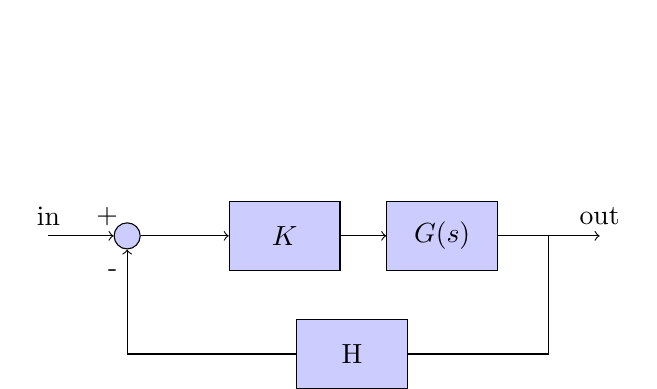
\begin{tikzpicture}[node distance = 2 cm]
  \node [input, name=input] {};
\node [sum,right of= input](sum) {};
\node [block, right of=sum] (K) {\(K\)};
\node [block, right of=K] (sys) {\(G(s)\)};
\node [output, right of= sys] (output){};

\draw[->] (input) -- node[pos=0.9, above] {+} (sum);
\draw[->] (sum) -- (K);
\draw[->] (K) -- (sys);
\draw[->] (sys) -- node[name=feedback] {} (output);

\node at (0,2) {} ;
\node at (0,-2) {} ;

\node[yshift=0.25cm] at (input) {in};
\node[yshift=0.25cm] at (output) {out};
\draw[->] (feedback.center) |- ++(-2.5,-1.5) node[block, name=H] {H};
\draw[->] (H) -| node[pos=0.9, left] {-} (sum);
  \end{tikzpicture}
  \caption{closed loop system}
\end{subfigure}\hfill
\begin{subfigure}[c]{0.4\textwidth}
\centering
  \begin{tikzpicture}
    \draw
      (0,-1) -- (0,1) node[above] {\(j\omega\)}
      (-4,0) -- (1,0) node[right] {\(\sigma\)}
    ;

    \node[pole] at (-1,0) {};
    \node[pole] at (-2,0) {} ;
    \node[pole] at (-3,0) {} ;
    
    \draw[dashed,->] (-2,0) -- (0,3.46);
    \draw[dashed,->] (-2,0) -- (0,-3.46);
    \draw (-1.5,0) arc(0:60:0.5);
    
    \draw[very thick] (-2,0) -- (-1.5,0) to[out=90, in=240] (-1,1.73) -- (0,3.46);
    \draw[very thick] (-1,0) -- (-1.5,0) to[out=-90, in=-240] (-1,-1.73) -- (0,-3.46);
    \draw[very thick,->] (-3,0) -- (-3.9,0);
  \end{tikzpicture}
  \caption{Root Locus}
\end{subfigure}
\caption{Topics introduced in ``student to student'' teaching about control theory}
\end{figure}

Root Locus was defined and it was shown how to read a Root Locus plot and how to draw it by hand. 
We talked about PID controllers and what the parameters meant. 
We talked about systems that uses PID in the real world.
We talked about ways to chose parameters for PID using the Zigler Nichols method.

\subsubsection{Evaluation}
A lot of topics were chosen and it was impossible to get explore a single topic withe the given time constraints.

This made it possible to give an overview so people with little to no prior knowledge of control theory could visualize what is possible and how to design a controller.

The used math was not explained in this session as all the students knew about this already.

This was well received and people seemed to follow the conclusions without going into detail about Laplas transforms and second order systems.

The illustrations used was either examples from book
% \footnote{Dorf and Bishop,
% 	Modern Control Systems,
% 	Prentice Hall, 
% 	12th edition, 
% 	2011.} 
\cite[page. 12]{Control_Theory} 
% \todo[inline]{Control theory S2S: Book name and numbers} 
or drawn myself.

There were a lot of questions during the presentation which shows that they were interested in the subject

The response to the session was that it was a bit more technical than they expected. 
But the pace was fine and it was easy to follow. 

 %first appendix should be input, rest should be include
\newpage
\subsection{Thomas Søndergaard Christensen}
As a part of Experts in Teams we were required to teach a topic relevant to the development process of our product to the team. My main field being robotics, I decided to teach the topic of robot motion planning. My goal was to give an overview of the basic techniques used to plan robot motion, as well as some of the difficulties that you may be faced with when planning robot motion.
\subsubsection{Session Topics}
Initially a (very) brief overview of the different types of robots was given, three examples were used: Robot arms from the automotive industry, simple robot vacuum cleaners and finally, a team of football-playing robots competing for the Robocup.
Two very commonly used terms in robotics are the work-space and configuration-space of a robot. Using the example of a robot capable of motion in 2D space I explained the usefulness and limitations of the two concepts. Additionally I explained (or attempted to) the implications to the configuration-space of adding an obstacle in the work-space of a robot.
Lastly I presented the wavefront algorithm, explaining its workings and showing examples of applications used in class.
\subsubsection{Evaluation}
\paragraph{Group:}~\\
Generally people found the structure of the teaching session logical and easily understood. Additionally, the examples given were well-received and made a good job of describing the concepts. Some hinted that the difficulty could have been increased without it being an issue.
\paragraph{Own Reflections:}~\\
When deciding what material to include and what not to include I found it difficult to determine what level i would be teaching at. Given the limited time of the presentation, I did not want to attempt teaching subjects that require that some knowledge about robotic motion is already present. While my team did not necessarily have knowledge about my chosen subject in advance, they had had courses dealing with similar issues prior to my teaching session.\\
My experience from earlier student-to-student teachings told me that there would be many questions during the session, this led me to choose to  limit the length of my presentation to roughly 30 minutes, allowing time for questions. However, not a single question was asked during the presentation, meaning that my session fell short of the allowed 45 minutes. In hindsight I should have included an extra topic in case of the event that no questions were asked.\\
In general I am satisfied with the outcome of my teaching session. I believe the information was relevant to the project at hand and it was well received by my team.

% \include{./content/Appendix/}
\end{document} 